
% Default to the notebook output style

    


% Inherit from the specified cell style.




    
\documentclass[11pt]{article}

    
    
    \usepackage[T1]{fontenc}
    % Nicer default font (+ math font) than Computer Modern for most use cases
    \usepackage{mathpazo}

    % Basic figure setup, for now with no caption control since it's done
    % automatically by Pandoc (which extracts ![](path) syntax from Markdown).
    \usepackage{graphicx}
    % We will generate all images so they have a width \maxwidth. This means
    % that they will get their normal width if they fit onto the page, but
    % are scaled down if they would overflow the margins.
    \makeatletter
    \def\maxwidth{\ifdim\Gin@nat@width>\linewidth\linewidth
    \else\Gin@nat@width\fi}
    \makeatother
    \let\Oldincludegraphics\includegraphics
    % Set max figure width to be 80% of text width, for now hardcoded.
    \renewcommand{\includegraphics}[1]{\Oldincludegraphics[width=.8\maxwidth]{#1}}
    % Ensure that by default, figures have no caption (until we provide a
    % proper Figure object with a Caption API and a way to capture that
    % in the conversion process - todo).
    \usepackage{caption}
    \DeclareCaptionLabelFormat{nolabel}{}
    \captionsetup{labelformat=nolabel}

    \usepackage{adjustbox} % Used to constrain images to a maximum size 
    \usepackage{xcolor} % Allow colors to be defined
    \usepackage{enumerate} % Needed for markdown enumerations to work
    \usepackage{geometry} % Used to adjust the document margins
    \usepackage{amsmath} % Equations
    \usepackage{amssymb} % Equations
    \usepackage{textcomp} % defines textquotesingle
    % Hack from http://tex.stackexchange.com/a/47451/13684:
    \AtBeginDocument{%
        \def\PYZsq{\textquotesingle}% Upright quotes in Pygmentized code
    }
    \usepackage{upquote} % Upright quotes for verbatim code
    \usepackage{eurosym} % defines \euro
    \usepackage[mathletters]{ucs} % Extended unicode (utf-8) support
    \usepackage[utf8x]{inputenc} % Allow utf-8 characters in the tex document
    \usepackage{fancyvrb} % verbatim replacement that allows latex
    \usepackage{grffile} % extends the file name processing of package graphics 
                         % to support a larger range 
    % The hyperref package gives us a pdf with properly built
    % internal navigation ('pdf bookmarks' for the table of contents,
    % internal cross-reference links, web links for URLs, etc.)
    \usepackage{hyperref}
    \usepackage{longtable} % longtable support required by pandoc >1.10
    \usepackage{booktabs}  % table support for pandoc > 1.12.2
    \usepackage[inline]{enumitem} % IRkernel/repr support (it uses the enumerate* environment)
    \usepackage[normalem]{ulem} % ulem is needed to support strikethroughs (\sout)
                                % normalem makes italics be italics, not underlines
    

    
    
    % Colors for the hyperref package
    \definecolor{urlcolor}{rgb}{0,.145,.698}
    \definecolor{linkcolor}{rgb}{.71,0.21,0.01}
    \definecolor{citecolor}{rgb}{.12,.54,.11}

    % ANSI colors
    \definecolor{ansi-black}{HTML}{3E424D}
    \definecolor{ansi-black-intense}{HTML}{282C36}
    \definecolor{ansi-red}{HTML}{E75C58}
    \definecolor{ansi-red-intense}{HTML}{B22B31}
    \definecolor{ansi-green}{HTML}{00A250}
    \definecolor{ansi-green-intense}{HTML}{007427}
    \definecolor{ansi-yellow}{HTML}{DDB62B}
    \definecolor{ansi-yellow-intense}{HTML}{B27D12}
    \definecolor{ansi-blue}{HTML}{208FFB}
    \definecolor{ansi-blue-intense}{HTML}{0065CA}
    \definecolor{ansi-magenta}{HTML}{D160C4}
    \definecolor{ansi-magenta-intense}{HTML}{A03196}
    \definecolor{ansi-cyan}{HTML}{60C6C8}
    \definecolor{ansi-cyan-intense}{HTML}{258F8F}
    \definecolor{ansi-white}{HTML}{C5C1B4}
    \definecolor{ansi-white-intense}{HTML}{A1A6B2}

    % commands and environments needed by pandoc snippets
    % extracted from the output of `pandoc -s`
    \providecommand{\tightlist}{%
      \setlength{\itemsep}{0pt}\setlength{\parskip}{0pt}}
    \DefineVerbatimEnvironment{Highlighting}{Verbatim}{commandchars=\\\{\}}
    % Add ',fontsize=\small' for more characters per line
    \newenvironment{Shaded}{}{}
    \newcommand{\KeywordTok}[1]{\textcolor[rgb]{0.00,0.44,0.13}{\textbf{{#1}}}}
    \newcommand{\DataTypeTok}[1]{\textcolor[rgb]{0.56,0.13,0.00}{{#1}}}
    \newcommand{\DecValTok}[1]{\textcolor[rgb]{0.25,0.63,0.44}{{#1}}}
    \newcommand{\BaseNTok}[1]{\textcolor[rgb]{0.25,0.63,0.44}{{#1}}}
    \newcommand{\FloatTok}[1]{\textcolor[rgb]{0.25,0.63,0.44}{{#1}}}
    \newcommand{\CharTok}[1]{\textcolor[rgb]{0.25,0.44,0.63}{{#1}}}
    \newcommand{\StringTok}[1]{\textcolor[rgb]{0.25,0.44,0.63}{{#1}}}
    \newcommand{\CommentTok}[1]{\textcolor[rgb]{0.38,0.63,0.69}{\textit{{#1}}}}
    \newcommand{\OtherTok}[1]{\textcolor[rgb]{0.00,0.44,0.13}{{#1}}}
    \newcommand{\AlertTok}[1]{\textcolor[rgb]{1.00,0.00,0.00}{\textbf{{#1}}}}
    \newcommand{\FunctionTok}[1]{\textcolor[rgb]{0.02,0.16,0.49}{{#1}}}
    \newcommand{\RegionMarkerTok}[1]{{#1}}
    \newcommand{\ErrorTok}[1]{\textcolor[rgb]{1.00,0.00,0.00}{\textbf{{#1}}}}
    \newcommand{\NormalTok}[1]{{#1}}
    
    % Additional commands for more recent versions of Pandoc
    \newcommand{\ConstantTok}[1]{\textcolor[rgb]{0.53,0.00,0.00}{{#1}}}
    \newcommand{\SpecialCharTok}[1]{\textcolor[rgb]{0.25,0.44,0.63}{{#1}}}
    \newcommand{\VerbatimStringTok}[1]{\textcolor[rgb]{0.25,0.44,0.63}{{#1}}}
    \newcommand{\SpecialStringTok}[1]{\textcolor[rgb]{0.73,0.40,0.53}{{#1}}}
    \newcommand{\ImportTok}[1]{{#1}}
    \newcommand{\DocumentationTok}[1]{\textcolor[rgb]{0.73,0.13,0.13}{\textit{{#1}}}}
    \newcommand{\AnnotationTok}[1]{\textcolor[rgb]{0.38,0.63,0.69}{\textbf{\textit{{#1}}}}}
    \newcommand{\CommentVarTok}[1]{\textcolor[rgb]{0.38,0.63,0.69}{\textbf{\textit{{#1}}}}}
    \newcommand{\VariableTok}[1]{\textcolor[rgb]{0.10,0.09,0.49}{{#1}}}
    \newcommand{\ControlFlowTok}[1]{\textcolor[rgb]{0.00,0.44,0.13}{\textbf{{#1}}}}
    \newcommand{\OperatorTok}[1]{\textcolor[rgb]{0.40,0.40,0.40}{{#1}}}
    \newcommand{\BuiltInTok}[1]{{#1}}
    \newcommand{\ExtensionTok}[1]{{#1}}
    \newcommand{\PreprocessorTok}[1]{\textcolor[rgb]{0.74,0.48,0.00}{{#1}}}
    \newcommand{\AttributeTok}[1]{\textcolor[rgb]{0.49,0.56,0.16}{{#1}}}
    \newcommand{\InformationTok}[1]{\textcolor[rgb]{0.38,0.63,0.69}{\textbf{\textit{{#1}}}}}
    \newcommand{\WarningTok}[1]{\textcolor[rgb]{0.38,0.63,0.69}{\textbf{\textit{{#1}}}}}
    
    
    % Define a nice break command that doesn't care if a line doesn't already
    % exist.
    \def\br{\hspace*{\fill} \\* }
    % Math Jax compatability definitions
    \def\gt{>}
    \def\lt{<}
    % Document parameters
    \title{Untitled}
    
    
    

    % Pygments definitions
    
\makeatletter
\def\PY@reset{\let\PY@it=\relax \let\PY@bf=\relax%
    \let\PY@ul=\relax \let\PY@tc=\relax%
    \let\PY@bc=\relax \let\PY@ff=\relax}
\def\PY@tok#1{\csname PY@tok@#1\endcsname}
\def\PY@toks#1+{\ifx\relax#1\empty\else%
    \PY@tok{#1}\expandafter\PY@toks\fi}
\def\PY@do#1{\PY@bc{\PY@tc{\PY@ul{%
    \PY@it{\PY@bf{\PY@ff{#1}}}}}}}
\def\PY#1#2{\PY@reset\PY@toks#1+\relax+\PY@do{#2}}

\expandafter\def\csname PY@tok@w\endcsname{\def\PY@tc##1{\textcolor[rgb]{0.73,0.73,0.73}{##1}}}
\expandafter\def\csname PY@tok@c\endcsname{\let\PY@it=\textit\def\PY@tc##1{\textcolor[rgb]{0.25,0.50,0.50}{##1}}}
\expandafter\def\csname PY@tok@cp\endcsname{\def\PY@tc##1{\textcolor[rgb]{0.74,0.48,0.00}{##1}}}
\expandafter\def\csname PY@tok@k\endcsname{\let\PY@bf=\textbf\def\PY@tc##1{\textcolor[rgb]{0.00,0.50,0.00}{##1}}}
\expandafter\def\csname PY@tok@kp\endcsname{\def\PY@tc##1{\textcolor[rgb]{0.00,0.50,0.00}{##1}}}
\expandafter\def\csname PY@tok@kt\endcsname{\def\PY@tc##1{\textcolor[rgb]{0.69,0.00,0.25}{##1}}}
\expandafter\def\csname PY@tok@o\endcsname{\def\PY@tc##1{\textcolor[rgb]{0.40,0.40,0.40}{##1}}}
\expandafter\def\csname PY@tok@ow\endcsname{\let\PY@bf=\textbf\def\PY@tc##1{\textcolor[rgb]{0.67,0.13,1.00}{##1}}}
\expandafter\def\csname PY@tok@nb\endcsname{\def\PY@tc##1{\textcolor[rgb]{0.00,0.50,0.00}{##1}}}
\expandafter\def\csname PY@tok@nf\endcsname{\def\PY@tc##1{\textcolor[rgb]{0.00,0.00,1.00}{##1}}}
\expandafter\def\csname PY@tok@nc\endcsname{\let\PY@bf=\textbf\def\PY@tc##1{\textcolor[rgb]{0.00,0.00,1.00}{##1}}}
\expandafter\def\csname PY@tok@nn\endcsname{\let\PY@bf=\textbf\def\PY@tc##1{\textcolor[rgb]{0.00,0.00,1.00}{##1}}}
\expandafter\def\csname PY@tok@ne\endcsname{\let\PY@bf=\textbf\def\PY@tc##1{\textcolor[rgb]{0.82,0.25,0.23}{##1}}}
\expandafter\def\csname PY@tok@nv\endcsname{\def\PY@tc##1{\textcolor[rgb]{0.10,0.09,0.49}{##1}}}
\expandafter\def\csname PY@tok@no\endcsname{\def\PY@tc##1{\textcolor[rgb]{0.53,0.00,0.00}{##1}}}
\expandafter\def\csname PY@tok@nl\endcsname{\def\PY@tc##1{\textcolor[rgb]{0.63,0.63,0.00}{##1}}}
\expandafter\def\csname PY@tok@ni\endcsname{\let\PY@bf=\textbf\def\PY@tc##1{\textcolor[rgb]{0.60,0.60,0.60}{##1}}}
\expandafter\def\csname PY@tok@na\endcsname{\def\PY@tc##1{\textcolor[rgb]{0.49,0.56,0.16}{##1}}}
\expandafter\def\csname PY@tok@nt\endcsname{\let\PY@bf=\textbf\def\PY@tc##1{\textcolor[rgb]{0.00,0.50,0.00}{##1}}}
\expandafter\def\csname PY@tok@nd\endcsname{\def\PY@tc##1{\textcolor[rgb]{0.67,0.13,1.00}{##1}}}
\expandafter\def\csname PY@tok@s\endcsname{\def\PY@tc##1{\textcolor[rgb]{0.73,0.13,0.13}{##1}}}
\expandafter\def\csname PY@tok@sd\endcsname{\let\PY@it=\textit\def\PY@tc##1{\textcolor[rgb]{0.73,0.13,0.13}{##1}}}
\expandafter\def\csname PY@tok@si\endcsname{\let\PY@bf=\textbf\def\PY@tc##1{\textcolor[rgb]{0.73,0.40,0.53}{##1}}}
\expandafter\def\csname PY@tok@se\endcsname{\let\PY@bf=\textbf\def\PY@tc##1{\textcolor[rgb]{0.73,0.40,0.13}{##1}}}
\expandafter\def\csname PY@tok@sr\endcsname{\def\PY@tc##1{\textcolor[rgb]{0.73,0.40,0.53}{##1}}}
\expandafter\def\csname PY@tok@ss\endcsname{\def\PY@tc##1{\textcolor[rgb]{0.10,0.09,0.49}{##1}}}
\expandafter\def\csname PY@tok@sx\endcsname{\def\PY@tc##1{\textcolor[rgb]{0.00,0.50,0.00}{##1}}}
\expandafter\def\csname PY@tok@m\endcsname{\def\PY@tc##1{\textcolor[rgb]{0.40,0.40,0.40}{##1}}}
\expandafter\def\csname PY@tok@gh\endcsname{\let\PY@bf=\textbf\def\PY@tc##1{\textcolor[rgb]{0.00,0.00,0.50}{##1}}}
\expandafter\def\csname PY@tok@gu\endcsname{\let\PY@bf=\textbf\def\PY@tc##1{\textcolor[rgb]{0.50,0.00,0.50}{##1}}}
\expandafter\def\csname PY@tok@gd\endcsname{\def\PY@tc##1{\textcolor[rgb]{0.63,0.00,0.00}{##1}}}
\expandafter\def\csname PY@tok@gi\endcsname{\def\PY@tc##1{\textcolor[rgb]{0.00,0.63,0.00}{##1}}}
\expandafter\def\csname PY@tok@gr\endcsname{\def\PY@tc##1{\textcolor[rgb]{1.00,0.00,0.00}{##1}}}
\expandafter\def\csname PY@tok@ge\endcsname{\let\PY@it=\textit}
\expandafter\def\csname PY@tok@gs\endcsname{\let\PY@bf=\textbf}
\expandafter\def\csname PY@tok@gp\endcsname{\let\PY@bf=\textbf\def\PY@tc##1{\textcolor[rgb]{0.00,0.00,0.50}{##1}}}
\expandafter\def\csname PY@tok@go\endcsname{\def\PY@tc##1{\textcolor[rgb]{0.53,0.53,0.53}{##1}}}
\expandafter\def\csname PY@tok@gt\endcsname{\def\PY@tc##1{\textcolor[rgb]{0.00,0.27,0.87}{##1}}}
\expandafter\def\csname PY@tok@err\endcsname{\def\PY@bc##1{\setlength{\fboxsep}{0pt}\fcolorbox[rgb]{1.00,0.00,0.00}{1,1,1}{\strut ##1}}}
\expandafter\def\csname PY@tok@kc\endcsname{\let\PY@bf=\textbf\def\PY@tc##1{\textcolor[rgb]{0.00,0.50,0.00}{##1}}}
\expandafter\def\csname PY@tok@kd\endcsname{\let\PY@bf=\textbf\def\PY@tc##1{\textcolor[rgb]{0.00,0.50,0.00}{##1}}}
\expandafter\def\csname PY@tok@kn\endcsname{\let\PY@bf=\textbf\def\PY@tc##1{\textcolor[rgb]{0.00,0.50,0.00}{##1}}}
\expandafter\def\csname PY@tok@kr\endcsname{\let\PY@bf=\textbf\def\PY@tc##1{\textcolor[rgb]{0.00,0.50,0.00}{##1}}}
\expandafter\def\csname PY@tok@bp\endcsname{\def\PY@tc##1{\textcolor[rgb]{0.00,0.50,0.00}{##1}}}
\expandafter\def\csname PY@tok@fm\endcsname{\def\PY@tc##1{\textcolor[rgb]{0.00,0.00,1.00}{##1}}}
\expandafter\def\csname PY@tok@vc\endcsname{\def\PY@tc##1{\textcolor[rgb]{0.10,0.09,0.49}{##1}}}
\expandafter\def\csname PY@tok@vg\endcsname{\def\PY@tc##1{\textcolor[rgb]{0.10,0.09,0.49}{##1}}}
\expandafter\def\csname PY@tok@vi\endcsname{\def\PY@tc##1{\textcolor[rgb]{0.10,0.09,0.49}{##1}}}
\expandafter\def\csname PY@tok@vm\endcsname{\def\PY@tc##1{\textcolor[rgb]{0.10,0.09,0.49}{##1}}}
\expandafter\def\csname PY@tok@sa\endcsname{\def\PY@tc##1{\textcolor[rgb]{0.73,0.13,0.13}{##1}}}
\expandafter\def\csname PY@tok@sb\endcsname{\def\PY@tc##1{\textcolor[rgb]{0.73,0.13,0.13}{##1}}}
\expandafter\def\csname PY@tok@sc\endcsname{\def\PY@tc##1{\textcolor[rgb]{0.73,0.13,0.13}{##1}}}
\expandafter\def\csname PY@tok@dl\endcsname{\def\PY@tc##1{\textcolor[rgb]{0.73,0.13,0.13}{##1}}}
\expandafter\def\csname PY@tok@s2\endcsname{\def\PY@tc##1{\textcolor[rgb]{0.73,0.13,0.13}{##1}}}
\expandafter\def\csname PY@tok@sh\endcsname{\def\PY@tc##1{\textcolor[rgb]{0.73,0.13,0.13}{##1}}}
\expandafter\def\csname PY@tok@s1\endcsname{\def\PY@tc##1{\textcolor[rgb]{0.73,0.13,0.13}{##1}}}
\expandafter\def\csname PY@tok@mb\endcsname{\def\PY@tc##1{\textcolor[rgb]{0.40,0.40,0.40}{##1}}}
\expandafter\def\csname PY@tok@mf\endcsname{\def\PY@tc##1{\textcolor[rgb]{0.40,0.40,0.40}{##1}}}
\expandafter\def\csname PY@tok@mh\endcsname{\def\PY@tc##1{\textcolor[rgb]{0.40,0.40,0.40}{##1}}}
\expandafter\def\csname PY@tok@mi\endcsname{\def\PY@tc##1{\textcolor[rgb]{0.40,0.40,0.40}{##1}}}
\expandafter\def\csname PY@tok@il\endcsname{\def\PY@tc##1{\textcolor[rgb]{0.40,0.40,0.40}{##1}}}
\expandafter\def\csname PY@tok@mo\endcsname{\def\PY@tc##1{\textcolor[rgb]{0.40,0.40,0.40}{##1}}}
\expandafter\def\csname PY@tok@ch\endcsname{\let\PY@it=\textit\def\PY@tc##1{\textcolor[rgb]{0.25,0.50,0.50}{##1}}}
\expandafter\def\csname PY@tok@cm\endcsname{\let\PY@it=\textit\def\PY@tc##1{\textcolor[rgb]{0.25,0.50,0.50}{##1}}}
\expandafter\def\csname PY@tok@cpf\endcsname{\let\PY@it=\textit\def\PY@tc##1{\textcolor[rgb]{0.25,0.50,0.50}{##1}}}
\expandafter\def\csname PY@tok@c1\endcsname{\let\PY@it=\textit\def\PY@tc##1{\textcolor[rgb]{0.25,0.50,0.50}{##1}}}
\expandafter\def\csname PY@tok@cs\endcsname{\let\PY@it=\textit\def\PY@tc##1{\textcolor[rgb]{0.25,0.50,0.50}{##1}}}

\def\PYZbs{\char`\\}
\def\PYZus{\char`\_}
\def\PYZob{\char`\{}
\def\PYZcb{\char`\}}
\def\PYZca{\char`\^}
\def\PYZam{\char`\&}
\def\PYZlt{\char`\<}
\def\PYZgt{\char`\>}
\def\PYZsh{\char`\#}
\def\PYZpc{\char`\%}
\def\PYZdl{\char`\$}
\def\PYZhy{\char`\-}
\def\PYZsq{\char`\'}
\def\PYZdq{\char`\"}
\def\PYZti{\char`\~}
% for compatibility with earlier versions
\def\PYZat{@}
\def\PYZlb{[}
\def\PYZrb{]}
\makeatother


    % Exact colors from NB
    \definecolor{incolor}{rgb}{0.0, 0.0, 0.5}
    \definecolor{outcolor}{rgb}{0.545, 0.0, 0.0}



    
    % Prevent overflowing lines due to hard-to-break entities
    \sloppy 
    % Setup hyperref package
    \hypersetup{
      breaklinks=true,  % so long urls are correctly broken across lines
      colorlinks=true,
      urlcolor=urlcolor,
      linkcolor=linkcolor,
      citecolor=citecolor,
      }
    % Slightly bigger margins than the latex defaults
    
    \geometry{verbose,tmargin=1in,bmargin=1in,lmargin=1in,rmargin=1in}
    
    

    \begin{document}
    
    
    \maketitle
    
    

    
    \section{Machine Learning Engineer
Nanodegree}\label{machine-learning-engineer-nanodegree}

\subsection{Capstone Project}\label{capstone-project}

Shane Moloney August 20th, 2018

\subsection{I. Definition}\label{i.-definition}

\subsubsection{Project Overview}\label{project-overview}

I found this project on Kaggle, the domain is underground probing by
seismic imaging and the processing of the resulting images to find salt
deposits. Areas of Earth with large quantities of oil and gas also
contain large deposits of salt, detecting these in the seismic images
currently requires experts to manually analyse all the images. This can
be very subjective, with varying conclusions, making it very difficult
to find the exact position of the deposits. Drilling an incorrect
position can cost huge amounts in wasted funds and worst of all, can
result in dangerous work conditions for the drilling crew. TGS is hoping
to use machine learning to find the deposits accurately and have
provided a large dataset of thousands of image samples and masks
containing the salt deposit locations. The competition and further
details can be found on the
\href{https://www.kaggle.com/c/tgs-salt-identification-challenge}{TGS
Salt Identification} competition page.

The dataset consists of greyscale images of seismic imaging data, there
are 4000 images provided for training and 18000 used for testing. A few
examples of the images can be seen below:\\
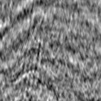
\includegraphics{pictures/example_0.png}
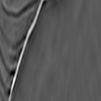
\includegraphics{pictures/example_1.png}
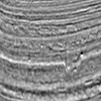
\includegraphics{pictures/example_2.png}
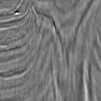
\includegraphics{pictures/example_3.png}

As you can see there are two types of material in the images. Sediment,
which appears in layers and horizontal stripes in the images, and salt,
which is flat or more chaotic in its structure in the images.

\subsubsection{Problem Statement}\label{problem-statement}

The problem is to identify the pixels that contain salt and produce a
mask of the image in which the pixel values range from 0 to 1 and these
values represent the probability of that pixel containing salt. This is
a problem that is perfect for a CNN, or specifically a Unet model CNN.
The Unet model is very effective at segmentation tasks and is known for
it's work on the
\href{https://lmb.informatik.uni-freiburg.de/people/ronneber/u-net/}{Biomedical
Image Segmentation} problem. The basis of this model is to reduce the
layer size exponentially and similarly increase the channel count until
the layer size reaches some minimum, ie. 32x32, and then to use
Conv2DTranspose layers to exponentially increase the layer sizes and
reduce the channel count to the original size. This allows for fast,
accurate image segmentation and has been used for many industries and
areas of study. A diagram of the Unet architecture that was used for the
Biomedical Image Segmentation problem can be seen below:

\begin{figure}
\centering
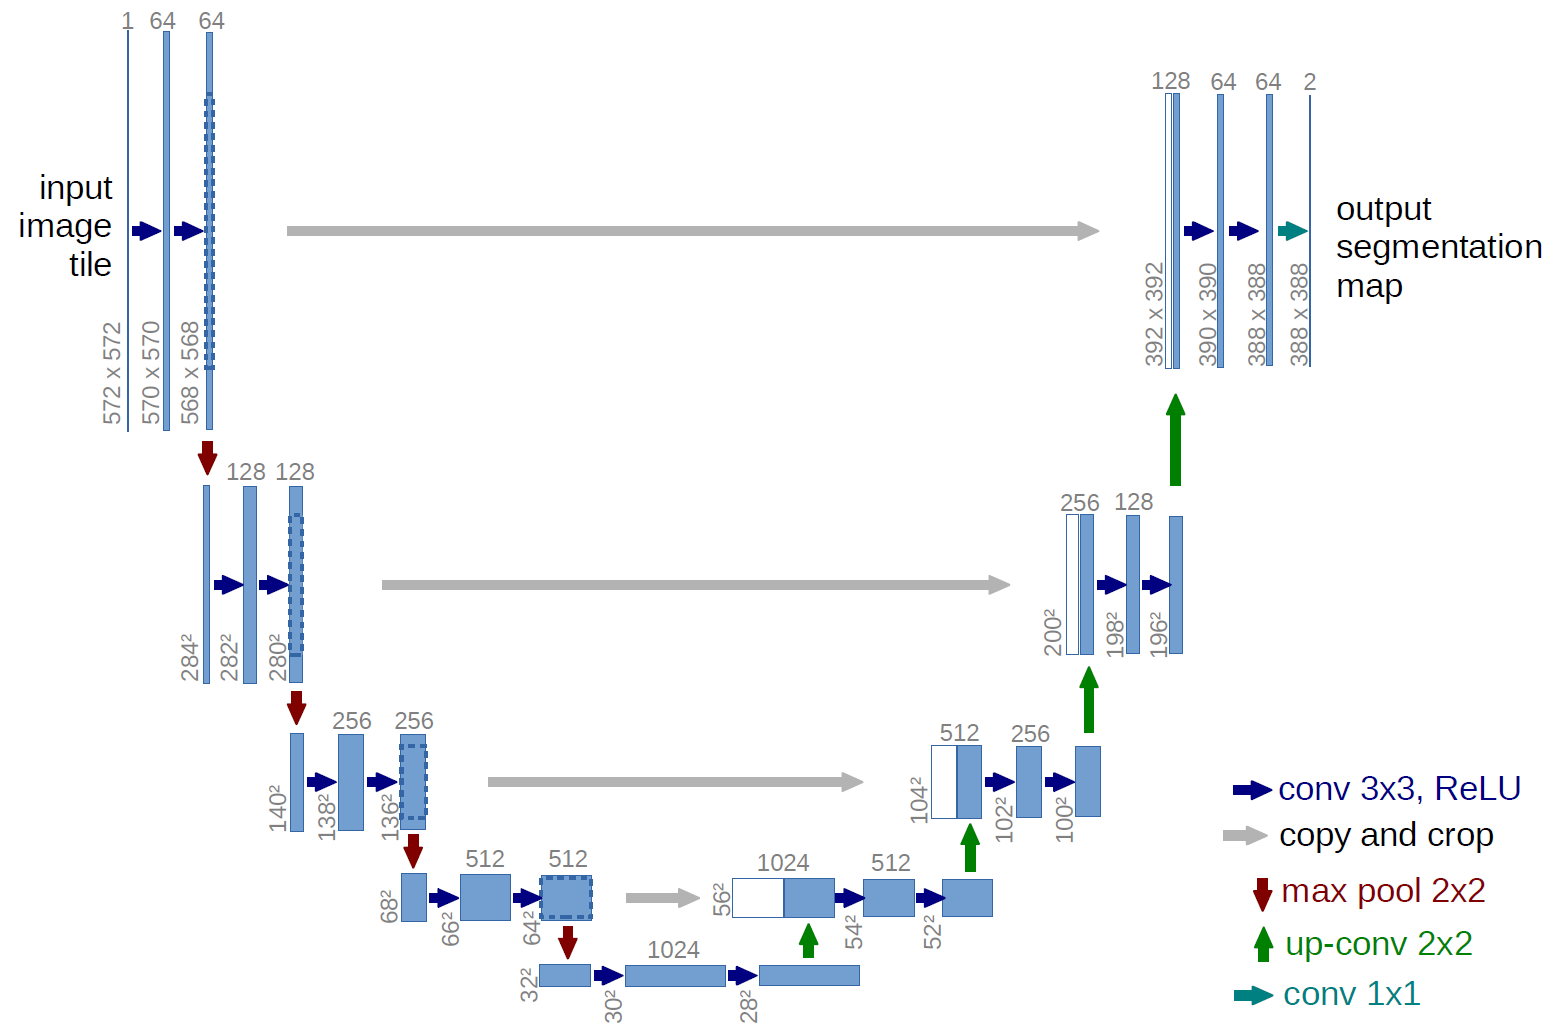
\includegraphics{pictures/u-net.png =100x100}
\caption{}
\end{figure}

This method should do relatively well without any additional methods
being used as this is a segmentation problem. There are many ways we can
improve the Unets results and the effectiveness of its training such as
data augmentation, dropout layers for network exploration, etc.

\subsubsection{Metrics}\label{metrics}

The evaluation for this challenge is done using the mean average
precision at different intersection over union thresholds. This is done
by first getting the prediction image A and the ground truth image B and
calculating their intersection over their union:

\[IoU(A, B) = \frac{A \bigcap B}{A \bigcup B}\]

The IoU is calculated based on a threshold, ie. if the threshold is 0.5
the IoU has to be over 0.5 to be considered a hit. The thresholds in
this case range from 0.5 to 0.95 with a step size of 0.05. For each
threshold, \(t\), we calculate a precision value using the number of
true positives (TP), false negatives (FN) and false positives (FP).
These are gathered when comparing the values of the prediction and the
ground truth:

\[\frac{TP_t}{TP_t + FP_t + FN_t}\]

The average precision value for a single image is calculated by the mean
of the precision values for each IoU threshold calculated above, so the
equation looks like this:

\[\frac{1}{thresholds}\sum_t\frac{TP_t}{TP_t + FP_t + FN_t}\]

Finally the models score is the mean of all the average precision values
of all the images in the test set.

\subsection{II. Analysis}\label{ii.-analysis}

\emph{(approx. 2-4 pages)}

\subsubsection{Data Exploration}\label{data-exploration}

I explored the data quite thoroughly in the notebook, but before I even
began properly analysing the data I found some interesting outliers.
After I imported the data I simply displayed the first five images and
their matching masks. These images can be seen below:
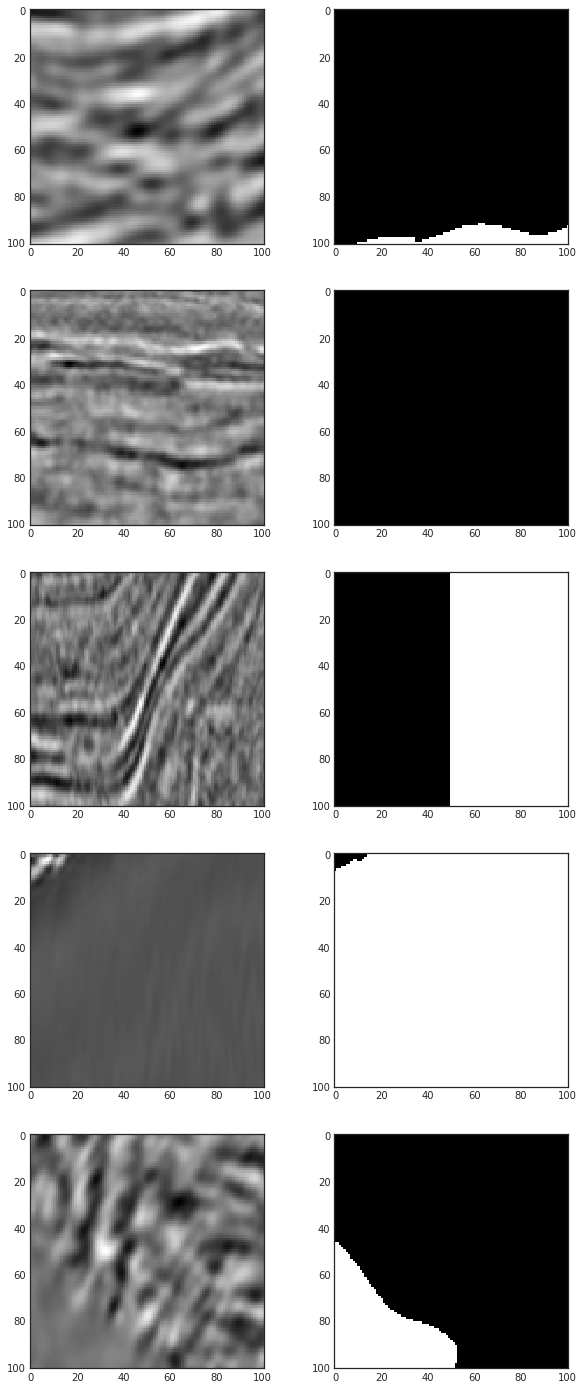
\includegraphics{pictures/first_five.png}

The issue should stand out immediately, the third images mask is a
perfectly straight border down the center of the image, I think this is
problematic as we want to train the model to accurately find the borders
between salt and sediment and I will explore this more in the Data
Preprocessing section below.

Next I began looking at the entire data by inspecting the coverage of
the salt in each image, or rather the percentage, between 0 and 1, of
the image that contains salt. This was calculated by simply by the
following method:

\[ cov = \frac{\sum_i pix}{w*h} \]

Now this is a continuous value which makes it difficult to group or
categorise images in this space so I created the coverage class column
where I apply a ceiling rounding policy to the discretisation. When we
plot these two columns from the data on a distribution plot we get the
following:

\begin{figure}
\centering
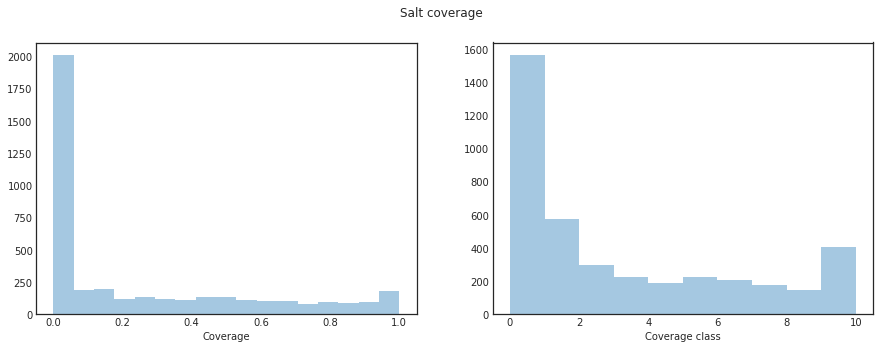
\includegraphics{pictures/coverage.png}
\caption{}
\end{figure}

Now we can see that approximately half the data set consists of images
with very little or no salt coverage. This is good as our model needs to
learn how to identify images with no salt as well as images with it.
There is another aspect to the data I hadn't mentioned yet, depth, the
data was accompanied with a CSV file containing the depths at which each
scan was taken, this is important to us as different depths would likely
result in different sediment and salt formations. Let's have a look at
the distribution of the depths sampled from both the training and
testing sets:

\begin{figure}
\centering
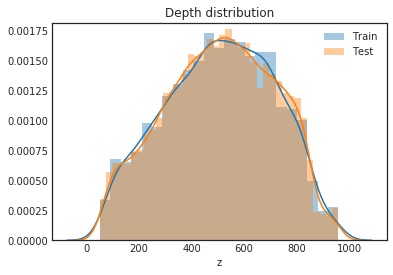
\includegraphics{pictures/depths.png}
\caption{}
\end{figure}

This looks like a nice gaussian distribution meaning we have a nice
random sampling of depths which is good for our training and gives us
more confidence in our ability to avoid overfitting to a specific data
set.

\subsubsection{Algorithms and
Techniques}\label{algorithms-and-techniques}

As explained above, I used the Unet model CNN for the main algorithm as
well as some data augmentation. For preprocessing I removed some
outliers that I will explain further below. I made use of early
stopping, model checkpointing and learning rate reduction when training
my model. - Early stopping: sets a maximum number of epochs where the
validation loss does not improve and once that limit is reached the
training endless - Model checkpointing: this simply saves the best
version of the model, so when the validation loss improves the current
weights are saved to a file to be retrieved after the training, by the
end of the training the file will contain the best models weights -
Learning rate reduction: when the improvement rate of the model begins
to slow, ie the validation loss stops improving, we reduce the learning
rate to make the changes in the weights less drastic and so zeros in on
the ideal weights faster

These were all used in conjunction with a high number of epochs and
batches.

\subsubsection{Benchmark}\label{benchmark}

While there is no benchmark model provided, a group has created an open
source project for this competition to be used as a benchmark or as
baseline code to be used as a space for experimentation or just to be
used as a starting off point. The project is being run by a group called
neptune.ml and can be found on their site
\href{https://app.neptune.ml/neptune-ml/Salt-Detection?namedFilterId=about}{here}.
I think this will make a good benchmark as it implements a Unet as well
and is not like other baseline code examples out there as the goal for
the project is to use an open source platform to work on the challenge
together so it does not stop at the most basic implementation and uses
augmentation and other methods to improve the score.

As is stated on their site, their first attempted solution scored 0.745,
which is to be expected of a solution developed by a community of people
interested or working in machine learning. I would be very impressed if
my solution is able to beat this as the top scores are just over 0.85
meaning there is only about a ten percent difference between the scores
and to bridge that gap would presumably require advanced, high level
machine learning knowledge.

\subsection{III. Methodology}\label{iii.-methodology}

\subsubsection{Data Preprocessing}\label{data-preprocessing}

There were three main parts to the data preprocessing: outlier removal,
resizing and augmentation.

\paragraph{Outlier Removal}\label{outlier-removal}

As we saw earlier there are some outliers where the masks have a
straight border between salt and sediment, this made me very suspicious
so I decided to inspect the entries with straight borders. I used OpenCV
to edge detect the masks and then rotated the image sideways, this
allowed me to simply iterate through the rows and find if there is a row
where all pixels were white. I applied this method to all the masks and
added the index of any straight bordered masks to an array.

\begin{Shaded}
\begin{Highlighting}[]
\KeywordTok{def}\NormalTok{ has_straight_border(mask_id, shape, edge_array):}
\NormalTok{    mask }\OperatorTok{=}\NormalTok{ cv2.imread(}\StringTok{'../input/train/masks/}\SpecialCharTok{\{\}}\StringTok{.png'}\NormalTok{.}\BuiltInTok{format}\NormalTok{(mask_id))}
\NormalTok{    edges }\OperatorTok{=}\NormalTok{ cv2.Canny(mask, }\DecValTok{100}\NormalTok{, }\DecValTok{200}\NormalTok{)}
\NormalTok{    mat }\OperatorTok{=}\NormalTok{ cv2.getRotationMatrix2D((shape[}\DecValTok{0}\NormalTok{]}\OperatorTok{/}\DecValTok{2}\NormalTok{,shape[}\DecValTok{1}\NormalTok{]}\OperatorTok{/}\DecValTok{2}\NormalTok{),}\DecValTok{90}\NormalTok{,}\DecValTok{1}\NormalTok{)}
\NormalTok{    edges_rotated }\OperatorTok{=}\NormalTok{ cv2.warpAffine(edges, mat, shape)}
\NormalTok{    edge_array.append(edges_rotated)}
    \ControlFlowTok{for}\NormalTok{ row }\KeywordTok{in}\NormalTok{ edges_rotated:}
        \ControlFlowTok{if} \BuiltInTok{all}\NormalTok{(pix }\OperatorTok{==} \DecValTok{255} \ControlFlowTok{for}\NormalTok{ pix }\KeywordTok{in}\NormalTok{ row):}
            \ControlFlowTok{return} \VariableTok{True}
    \ControlFlowTok{return} \VariableTok{False}
\end{Highlighting}
\end{Shaded}

There are 117 straight edged masks, I displayed all of these masks as
green overlays on their corresponding images to see what the cause might
be, a sample of these can be seen in the figure below:

\begin{figure}
\centering
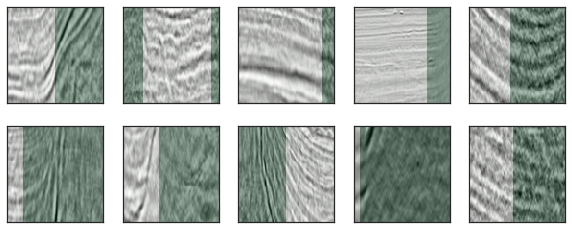
\includegraphics{pictures/straight.png}
\caption{}
\end{figure}

These borders are clearly not particularly accurate and seem to be broad
stroke feature identification. These need to be removed to prevent using
too many false positives and false negatives when training the model but
There are some that have a large salt coverage and we don't want to lose
that data. So I filtered the array based on the coverage class, only
keeping the images with a class of 8 or higher, this resulted in the
removal of 75 data points. We now have a dataset with shape
\texttt{(3925,\ 5)}.

\paragraph{Resizing}\label{resizing}

The Unet model, as explained earlier, exponentially decreases the size
of the convolutional layers, this means our inputs must have dimensions
that are a power of 2. So I created a function to upscale the images,
\texttt{upsample}, from their size of 101x101 to 128x128 and vice versa,
\texttt{downsample}. I then used these functions when creating the
training, testing and validation sets:

\begin{Shaded}
\begin{Highlighting}[]
\NormalTok{train_test_split(}
\NormalTok{    train_idx,}
\NormalTok{    np.array(train_full.images.}\BuiltInTok{map}\NormalTok{(upsample).tolist()).reshape(}\OperatorTok{-}\DecValTok{1}\NormalTok{, new_size, new_size, }\DecValTok{1}\NormalTok{),}
\NormalTok{    np.array(train_full.masks.}\BuiltInTok{map}\NormalTok{(upsample).tolist()).reshape(}\OperatorTok{-}\DecValTok{1}\NormalTok{, new_size, new_size, }\DecValTok{1}\NormalTok{),}
\NormalTok{    train_full.coverage.values,}
\NormalTok{    train_full.z.values,}
\NormalTok{    test_size}\OperatorTok{=}\FloatTok{0.2}\NormalTok{, stratify}\OperatorTok{=}\NormalTok{train_full.coverage_class, random_state}\OperatorTok{=}\DecValTok{117}\NormalTok{)}
\end{Highlighting}
\end{Shaded}

I also used the coverage class attribute of the data as a stratification
criterion to ensure an even spread of the different types of images. The
outputs from this function is a training and test set for the The data
sets now contained upscaled versions of the images and masks:

\begin{figure}
\centering
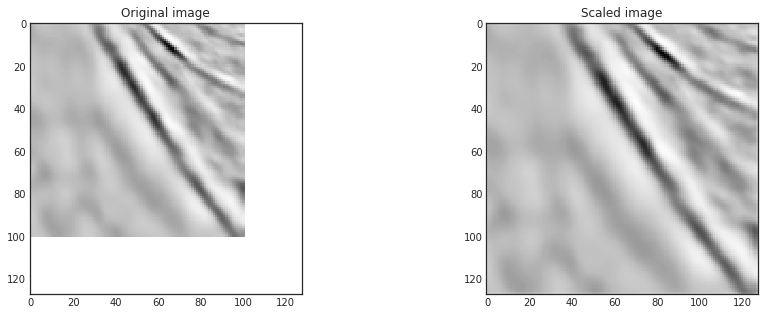
\includegraphics{pictures/upscaled.png}
\caption{}
\end{figure}

\paragraph{Data Augmentation}\label{data-augmentation}

Finally I augmented the data by simply flipping the x-axis on each of
the images and masks, this is because with a data set such as this,
where all of the segmentation subjects are naturally occurring phenomena
there will be no two images that are exactly the same. This means that
flipping the images essentially doubles our data for training and
testing. This was done with a simple line of code:

\begin{Shaded}
\begin{Highlighting}[]
\NormalTok{train_x }\OperatorTok{=}\NormalTok{ np.append(train_x, [np.fliplr(img) }\ControlFlowTok{for}\NormalTok{ img }\KeywordTok{in}\NormalTok{ train_x], axis}\OperatorTok{=}\DecValTok{0}\NormalTok{)}
\NormalTok{train_y }\OperatorTok{=}\NormalTok{ np.append(train_y, [np.fliplr(img) }\ControlFlowTok{for}\NormalTok{ img }\KeywordTok{in}\NormalTok{ train_y], axis}\OperatorTok{=}\DecValTok{0}\NormalTok{)}
\end{Highlighting}
\end{Shaded}

\begin{figure}
\centering
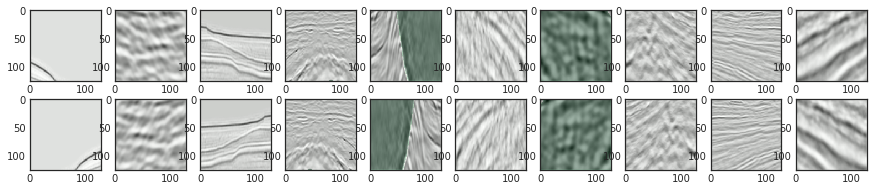
\includegraphics{pictures/flipped.png}
\caption{}
\end{figure}

\subsubsection{Implementation}\label{implementation}

The model itself I placed inside a function so I could easily edit the
parameters and experiment with different values. The function takes in
the input layer and the number of channels to begin with, again this
should be a power of two. I also set up variables within the function
for dropout, kernel and stride:

\begin{Shaded}
\begin{Highlighting}[]
\KeywordTok{def}\NormalTok{ build_model(input_layer, base_channels):}
\NormalTok{    dropout }\OperatorTok{=} \FloatTok{0.25}
\NormalTok{    kernel }\OperatorTok{=}\NormalTok{ (}\DecValTok{3}\NormalTok{, }\DecValTok{3}\NormalTok{)}
\NormalTok{    stride }\OperatorTok{=}\NormalTok{ (}\DecValTok{2}\NormalTok{, }\DecValTok{2}\NormalTok{)}
    \CommentTok{# Image size: 128 to 64}
\NormalTok{    conv1 }\OperatorTok{=}\NormalTok{ Conv2D(base_channels, kernel, activation}\OperatorTok{=}\StringTok{"relu"}\NormalTok{, padding}\OperatorTok{=}\StringTok{"same"}\NormalTok{)(input_layer)}
\NormalTok{    conv1 }\OperatorTok{=}\NormalTok{ Conv2D(base_channels, kernel, activation}\OperatorTok{=}\StringTok{"relu"}\NormalTok{, padding}\OperatorTok{=}\StringTok{"same"}\NormalTok{)(conv1)}
\NormalTok{    pool1 }\OperatorTok{=}\NormalTok{ MaxPooling2D((}\DecValTok{2}\NormalTok{, }\DecValTok{2}\NormalTok{))(conv1)}
\NormalTok{    pool1 }\OperatorTok{=}\NormalTok{ Dropout(dropout)(pool1)}

    \CommentTok{# Image size: 64 to 32}
\NormalTok{    conv2 }\OperatorTok{=}\NormalTok{ Conv2D(base_channels }\OperatorTok{*} \DecValTok{2}\NormalTok{, kernel, activation}\OperatorTok{=}\StringTok{"relu"}\NormalTok{, padding}\OperatorTok{=}\StringTok{"same"}\NormalTok{)(pool1)}
\NormalTok{    conv2 }\OperatorTok{=}\NormalTok{ Conv2D(base_channels }\OperatorTok{*} \DecValTok{2}\NormalTok{, kernel, activation}\OperatorTok{=}\StringTok{"relu"}\NormalTok{, padding}\OperatorTok{=}\StringTok{"same"}\NormalTok{)(conv2)}
\NormalTok{    pool2 }\OperatorTok{=}\NormalTok{ MaxPooling2D((}\DecValTok{2}\NormalTok{, }\DecValTok{2}\NormalTok{))(conv2)}
\NormalTok{    pool2 }\OperatorTok{=}\NormalTok{ Dropout(dropout}\OperatorTok{*}\DecValTok{2}\NormalTok{)(pool2)}

    \CommentTok{# Image size: 32 to 16}
\NormalTok{    conv3 }\OperatorTok{=}\NormalTok{ Conv2D(base_channels }\OperatorTok{*} \DecValTok{4}\NormalTok{, kernel, activation}\OperatorTok{=}\StringTok{"relu"}\NormalTok{, padding}\OperatorTok{=}\StringTok{"same"}\NormalTok{)(pool2)}
\NormalTok{    conv3 }\OperatorTok{=}\NormalTok{ Conv2D(base_channels }\OperatorTok{*} \DecValTok{4}\NormalTok{, kernel, activation}\OperatorTok{=}\StringTok{"relu"}\NormalTok{, padding}\OperatorTok{=}\StringTok{"same"}\NormalTok{)(conv3)}
\NormalTok{    pool3 }\OperatorTok{=}\NormalTok{ MaxPooling2D((}\DecValTok{2}\NormalTok{, }\DecValTok{2}\NormalTok{))(conv3)}
\NormalTok{    pool3 }\OperatorTok{=}\NormalTok{ Dropout(dropout}\OperatorTok{*}\DecValTok{2}\NormalTok{)(pool3)}

    \CommentTok{# Image size: 16 to 8}
\NormalTok{    conv4 }\OperatorTok{=}\NormalTok{ Conv2D(base_channels }\OperatorTok{*} \DecValTok{8}\NormalTok{, kernel, activation}\OperatorTok{=}\StringTok{"relu"}\NormalTok{, padding}\OperatorTok{=}\StringTok{"same"}\NormalTok{)(pool3)}
\NormalTok{    conv4 }\OperatorTok{=}\NormalTok{ Conv2D(base_channels }\OperatorTok{*} \DecValTok{8}\NormalTok{, kernel, activation}\OperatorTok{=}\StringTok{"relu"}\NormalTok{, padding}\OperatorTok{=}\StringTok{"same"}\NormalTok{)(conv4)}
\NormalTok{    pool4 }\OperatorTok{=}\NormalTok{ MaxPooling2D((}\DecValTok{2}\NormalTok{, }\DecValTok{2}\NormalTok{))(conv4)}
\NormalTok{    pool4 }\OperatorTok{=}\NormalTok{ Dropout(dropout}\OperatorTok{*}\DecValTok{2}\NormalTok{)(pool4)}

    \CommentTok{# Midway point}
\NormalTok{    conv_mid }\OperatorTok{=}\NormalTok{ Conv2D(base_channels }\OperatorTok{*} \DecValTok{16}\NormalTok{, kernel, activation}\OperatorTok{=}\StringTok{"relu"}\NormalTok{, padding}\OperatorTok{=}\StringTok{"same"}\NormalTok{)(pool4)}
\NormalTok{    conv_mid }\OperatorTok{=}\NormalTok{ Conv2D(base_channels }\OperatorTok{*} \DecValTok{16}\NormalTok{, kernel, activation}\OperatorTok{=}\StringTok{"relu"}\NormalTok{, padding}\OperatorTok{=}\StringTok{"same"}\NormalTok{)(conv_mid)}

    \CommentTok{# Now we mirror the above layers and begin increasing the image size using Conv2DTranspose layers}
    \CommentTok{# Image size: 8 to 16}
\NormalTok{    trans_conv4 }\OperatorTok{=}\NormalTok{ Conv2DTranspose(base_channels }\OperatorTok{*} \DecValTok{8}\NormalTok{, kernel, strides}\OperatorTok{=}\NormalTok{stride, padding}\OperatorTok{=}\StringTok{"same"}\NormalTok{)(conv_mid)}
\NormalTok{    uconv4 }\OperatorTok{=}\NormalTok{ concatenate([trans_conv4, conv4])}
\NormalTok{    uconv4 }\OperatorTok{=}\NormalTok{ Dropout(dropout }\OperatorTok{*} \DecValTok{2}\NormalTok{)(uconv4)}
\NormalTok{    uconv4 }\OperatorTok{=}\NormalTok{ Conv2D(base_channels }\OperatorTok{*} \DecValTok{8}\NormalTok{, kernel, activation}\OperatorTok{=}\StringTok{"relu"}\NormalTok{, padding}\OperatorTok{=}\StringTok{"same"}\NormalTok{)(uconv4)}
\NormalTok{    uconv4 }\OperatorTok{=}\NormalTok{ Conv2D(base_channels }\OperatorTok{*} \DecValTok{8}\NormalTok{, kernel, activation}\OperatorTok{=}\StringTok{"relu"}\NormalTok{, padding}\OperatorTok{=}\StringTok{"same"}\NormalTok{)(uconv4)}

    \CommentTok{# Image size: 16 to 32}
\NormalTok{    trans_conv3 }\OperatorTok{=}\NormalTok{ Conv2DTranspose(base_channels }\OperatorTok{*} \DecValTok{4}\NormalTok{, kernel, strides}\OperatorTok{=}\NormalTok{stride, padding}\OperatorTok{=}\StringTok{"same"}\NormalTok{)(uconv4)}
\NormalTok{    uconv3 }\OperatorTok{=}\NormalTok{ concatenate([trans_conv3, conv3])}
\NormalTok{    uconv3 }\OperatorTok{=}\NormalTok{ Dropout(dropout }\OperatorTok{*} \DecValTok{2}\NormalTok{)(uconv3)}
\NormalTok{    uconv3 }\OperatorTok{=}\NormalTok{ Conv2D(base_channels }\OperatorTok{*} \DecValTok{4}\NormalTok{, kernel, activation}\OperatorTok{=}\StringTok{"relu"}\NormalTok{, padding}\OperatorTok{=}\StringTok{"same"}\NormalTok{)(uconv3)}
\NormalTok{    uconv3 }\OperatorTok{=}\NormalTok{ Conv2D(base_channels }\OperatorTok{*} \DecValTok{4}\NormalTok{, kernel, activation}\OperatorTok{=}\StringTok{"relu"}\NormalTok{, padding}\OperatorTok{=}\StringTok{"same"}\NormalTok{)(uconv3)}

    \CommentTok{# Image size: 32 to 64}
\NormalTok{    trans_conv2 }\OperatorTok{=}\NormalTok{ Conv2DTranspose(base_channels }\OperatorTok{*} \DecValTok{2}\NormalTok{, kernel, strides}\OperatorTok{=}\NormalTok{stride, padding}\OperatorTok{=}\StringTok{"same"}\NormalTok{)(uconv3)}
\NormalTok{    uconv2 }\OperatorTok{=}\NormalTok{ concatenate([trans_conv2, conv2])}
\NormalTok{    uconv2 }\OperatorTok{=}\NormalTok{ Dropout(dropout }\OperatorTok{*} \DecValTok{2}\NormalTok{)(uconv2)}
\NormalTok{    uconv2 }\OperatorTok{=}\NormalTok{ Conv2D(base_channels }\OperatorTok{*} \DecValTok{2}\NormalTok{, kernel, activation}\OperatorTok{=}\StringTok{"relu"}\NormalTok{, padding}\OperatorTok{=}\StringTok{"same"}\NormalTok{)(uconv2)}
\NormalTok{    uconv2 }\OperatorTok{=}\NormalTok{ Conv2D(base_channels }\OperatorTok{*} \DecValTok{2}\NormalTok{, kernel, activation}\OperatorTok{=}\StringTok{"relu"}\NormalTok{, padding}\OperatorTok{=}\StringTok{"same"}\NormalTok{)(uconv2)}

    \CommentTok{# Image size: 64 to 128}
\NormalTok{    trans_conv1 }\OperatorTok{=}\NormalTok{ Conv2DTranspose(base_channels, kernel, strides}\OperatorTok{=}\NormalTok{stride, padding}\OperatorTok{=}\StringTok{"same"}\NormalTok{)(uconv2)}
\NormalTok{    uconv1 }\OperatorTok{=}\NormalTok{ concatenate([trans_conv1, conv1])}
\NormalTok{    uconv1 }\OperatorTok{=}\NormalTok{ Dropout(dropout)(uconv1)}
\NormalTok{    uconv1 }\OperatorTok{=}\NormalTok{ Conv2D(base_channels, kernel, activation}\OperatorTok{=}\StringTok{"relu"}\NormalTok{, padding}\OperatorTok{=}\StringTok{"same"}\NormalTok{)(uconv1)}
\NormalTok{    uconv1 }\OperatorTok{=}\NormalTok{ Conv2D(base_channels, kernel, activation}\OperatorTok{=}\StringTok{"relu"}\NormalTok{, padding}\OperatorTok{=}\StringTok{"same"}\NormalTok{)(uconv1)}

\NormalTok{    output_layer }\OperatorTok{=}\NormalTok{ Conv2D(}\DecValTok{1}\NormalTok{, (}\DecValTok{1}\NormalTok{, }\DecValTok{1}\NormalTok{), padding}\OperatorTok{=}\StringTok{"same"}\NormalTok{, activation}\OperatorTok{=}\StringTok{"sigmoid"}\NormalTok{)(uconv1)}

    \ControlFlowTok{return}\NormalTok{ output_layer}
\end{Highlighting}
\end{Shaded}

\subsubsection{Refinement}\label{refinement}

Above is the final version of the function, but I spent a lot of time
experimenting with different values for the various parameters,
especially \texttt{dropout} and \texttt{base\_channels} to try and find
the ideal combination. Originally I used just the base Unet model with
no dropout and only starting with 2 channels, as I understood more about
how the model functions I added the dropout layers, refined their use to
what you see above of increasing dropout in the inner layers and
decreasing in the first and final layers. This exploration helped
immensely as the Unet model reaches a very large amount of channels and
so can easily end up ignoring some due to early weight imbalances.

I also tried different optimizers and loss parameters, but the hardest
variables to experiment with were the early stopping and learning rate
reduction thresholds as these had a drastic effect on training time and
were the most time consuming to refine.

\subsection{IV. Results}\label{iv.-results}

\emph{(approx. 2-3 pages)}

\subsubsection{Model Evaluation and
Validation}\label{model-evaluation-and-validation}

The first thing I did after running my model was plot the validation and
training loss against one another as well as the accuracy, it was very
apparent where the ideal model lay in each training due to the
separation of the two scores as the model began to overfit to the
training data:

\begin{figure}
\centering
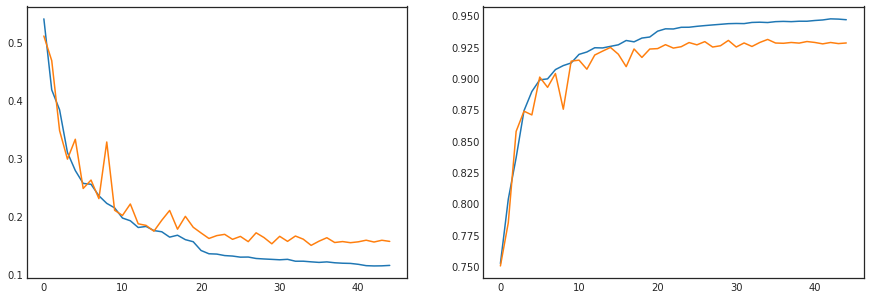
\includegraphics{pictures/validation.png}
\caption{}
\end{figure}

The next thing I did was do a sanity check using the validation set, I
predicted the set and displayed them on top of the images and masks as
seen previously, where grey is the original image, green is the ground
truth and red is the prediction. The red varies in severity as the model
produces probabilities so the lighter the red the less likely the model
considers that pixel to be salt.

\begin{figure}
\centering
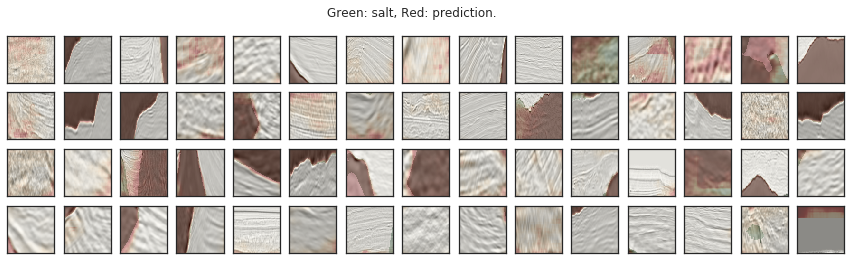
\includegraphics{pictures/predictions.png}
\caption{}
\end{figure}

The model did very well in a majority of the images, you can see it
produced a clear border between the salt and the sediment and was very
sure of the salt pattern inside the borders. It also sometimes seems to
try hard to find salt where there isn't any, on a few images we can see
the model has placed low probabilities throughout when there is no salt,
while on other zero coverage images it is sure that there is no salt.
The model also seems to struggle if there are multiple borders in the
one image, ie if there is a layer of salt inlayed throughout the
sediment as opposed to a single border split, the same applies vice
versa as we can see that images with a column of sediment flanked either
side by salt, the model predicts one but not both of the salt segments.
This could be due to a lack of such images in the training data, or a
the very least a minority of some such images.

Next I ran the IoU metrics and used the thresholds provided by the
competition. As defined in the metrics section of this report the IoU is
calculated for each image and each threshold, the final score is the
average of all these values. In our case we are going to look at a graph
of the IoU score for each threshold:

\begin{figure}
\centering
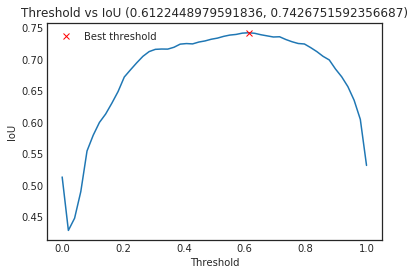
\includegraphics{pictures/IoU.png}
\caption{}
\end{figure}

The graph shows a wide curve where the low thresholds produces a low
score due to the very low probability pixels being counted as salt
predictions. The high thresholds also score lower as only pixels the
model is very sure of are counted and so this leaves very little room
for error. As we can see the model does best when the threshold is set
to only count pixels as salt predictions with an IoU of
\textasciitilde{}0.4 -\textgreater{} \textasciitilde{}0.7. The goal is
to make this curve as tall and as wide as possible since the end metric
is the average of all these scores. In this run the best threshold was
\textasciitilde{}0.612, the model received an IoU score of
\textasciitilde{}0.743 at this threshold, but what does this mean? We
can visualise the difference between the thresholded predictions and the
unrestricted predictions by displaying the same images as above but with
the prediction threshold set to the best performing one of
\textasciitilde{}0.612:

\begin{figure}
\centering
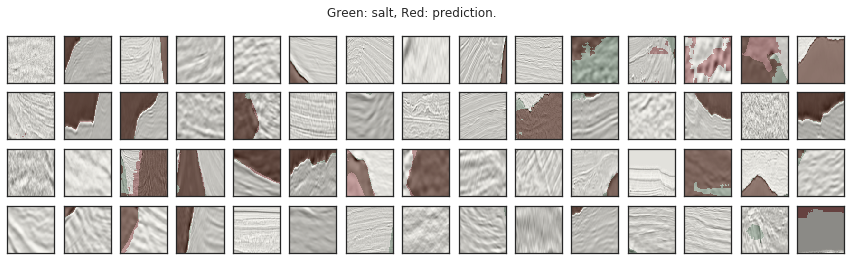
\includegraphics{pictures/thresh-IoU.png}
\caption{}
\end{figure}

Here we can see that the edges become even more clear, any pixels with a
probability value of less than the threshold are gone, this improves
many predictions by removing the fuzzy edges and providing a more
precise segmentation of the salt deposits. It can also worsen other
predictions as we can see where the model was unsure but correct about a
deposit that prediction has not been counted. All in all this threshold
produces a much cleaner prediction and we can see the model performs
very well with this threshold applied.

Finally I run my predictions on the test set, this set is 18000 images
and all the predictions must be run-length encoded for the submission
file for the competition. This is a simple enough function that
everybody in the competition needed so I use the one written by
\href{https://www.kaggle.com/bguberfain/unet-with-depth}{bguberfain}.
The file is submitted and I received a score of 0.716, which places me
at 792nd out of 1375 entrants. I think my model did very well
considering it was up against machine learning experts and experienced
ML engineers from around the world, but also because I think even if a
machine learning model was deployed in this industry it would still be
necessary to have an expert double check positive predictions. Even my
model seems to correctly predict the existence of the salt deposit quite
well and seems like it might only struggle with small deposits.

\subsubsection{Justification}\label{justification}

As stated above the benchmark model got a score of 0.745 and has
continued to improve but I am using their first solutions score as it
only seems fair given it is an open source project that is continuously
going to improve. While my model scored 0.716, meaning there is a
difference of only \textasciitilde{}0.02 between my score and the
benchmarks, I consider this to be a great result as a new member of the
machine learning community. If I had more time I would like to continue
to improve upon my method and find new techniques and algorithms to help
refine both my model and my processes for coming up with it.

\subsection{V. Conclusion}\label{v.-conclusion}

\subsubsection{Reflection}\label{reflection}

I found the whole process very interesting, the exploration of the data
involved a lot of experimentation and taught me a lot about both data
exploration and provided some great pyplot experience. I learned a lot
about seismic image segmentation, mostly I learned about it when
searching for a benchmark model and read through a few academic articles
which taught me a lot about sediment, and salt deposits. On top of that
my research into CNNs and then into Unets was very interesting and
really enhanced my knowledge of neural networks as a whole. I discovered
Unets from the competitions community where I saw the titles of many
kernels and submissions were "Unet with ...", this caused me to look up
what a Unet was and how to use them, I could immediately see why they
were a common solution attempt for competitors as they are designed for
segmentation tasks.

The most difficult part of the process I found was to be the refinement
of and experimentation with the model training parameters just due to
how long it takes to train and how many different parameters and
variables are involved in tuning the model. Evaluating the model was
very easy though as the metrics were so well defined and there were many
different ways to examine the models performance. The thresholds graph
provided a clear view of the general performance and allows us to easily
see improvements or shortcomings of the model.

The final solution definitely has room for improvement and if the goal
was to simply find salt deposits as opposed to accurately mapping them I
believe this model could be used but currently as the latter is the
problem posed I don't believe my model could be used in this space. I
learned a lot over the course of the project and am glad I could pursue
such an interesting problem statement and explore a domain I had no
previous experience or knowledge of.

\subsubsection{Improvement}\label{improvement}

I think my methods could definitely be improved, the outlier
identification and removal could perhaps be handled better or be made
more robust. I think there may be more I can do with the preprocessing
of the data, such as incorporating the depth in some way, such as
colouring the images based on their depth as it may be an important
feature in a salt deposits identification. Of course there can always be
more tweaking of the training parameters and the model itself to find
the ideal set up. While I don't know of any other methods or techniques
that could be used I am sure there are plenty out there that could
vastly improve my model but I didn't have time to truly research
anything that the course hadn't already mentioned or I wasn't already
aware of in some capacity.

If I were to use my solution as a new benchmark I think I could improve
upon it, I know there are many better solutions due to the leaderboard
on the competition page which likely make used of advanced ML techniques
or combinations of methods that I never even considered.


    % Add a bibliography block to the postdoc
    
    
    
    \end{document}
